\section{Delegated Quantum Computation (DQC) experiment on NV}
\label{qnodeos:sec:delcomp}

\subsection{Procedure}

We execute the application in a tomography way to establish \ac{QNodeOS} the quantum performance metric (\cref{qnodeos:fig:fig3}b, where we use $P_c$ to refer to the client program, and $P_s$ to the server program): The client \ac{CNPU} initiates $P_c$ with fixed $(\alpha, \theta)$. This results in a single \ac{CNPU} process, a single \ac{QNPU} process, and opening of an \ac{ER} socket (see \cref{qnodeos:sec:design_er_socket}) with the server node. At the same time, the server \ac{CNPU} initiates $P_s$ resulting in single \ac{CNPU} process, a single \ac{QNPU} process, and opening of an \ac{ER} socket with the client node. The client and the server programs execute the subroutines in \cref{qnodeos:fig:fig3}c, looping 1200 times: both immediately start the second iteration once the first is completed. After the 1200th iteration, both client and server stop their respective \ac{CNPU} and \ac{QNPU} processes. Source code including compiled NetQASM subroutines is available in \cref{qnodeos:sec:app_source}. We repeat 6 times for $(\alpha, \theta) \in \{\pi/2, \pi\} \times \{\pi/4, \pi/2, \pi\}$ for a total of 7200 executions of the circuit depicted in \cref{qnodeos:fig:fig3}a. We expect $\ket{\psi}$ to be either $\ket{-Y}$ (for $\alpha = \pi/2$) or $\ket{-Z}$ (for $\alpha = \pi$). To estimate the resulting $\ket{\psi}$ per $(\alpha, \theta)$, the contents of S2 (containing the server qubit measurement) in the server loop is was varied such that we obtained 600 measurement outcomes in basis $\ket{+Y}$ ($\ket{+Z}$) and 600 measurement outcomes in the corresponding orthogonal basis $\ket{-Y}$ ($\ket{-Z}$) for $\alpha = \pi/2$ ($\pi$).

Since our experiments are conducted on two \ac{NV} nodes that are directly connected, we install a constant network schedule with time-bins of 10\,ms in which all time-bins are assigned to networking. This allows us to assess the performance of executing quantum network applications without introducing a dependence on changing network schedules. This means the network process is made ready at the start of each such time-bin, although may not instruct the \ac{QDevice} to make entanglement if no requests for entanglement have been made.

\subsection{Definitions}

The result of a single \ac{DQC} circuit execution (\cref{qnodeos:fig:fig3}a) is a single-qubit state $\rho_{\text{DQC}}$ on the server. The success of running \ac{DQC} can be expressed as the fidelity of $\rho_{\text{DQC}}$ compared to the expected state (in case of no noise) $\ket{\psi}$ (\cref{qnodeos:fig:fig3}a). In the following we will call this fidelity the \ac{DQC} fidelity, or $F_{\text{DQC}}$.

The value of $F_{\text{DQC}}$ is affected the most by (1) the fidelity $F_{\text{EPR}}$ of the entangled pair created between the client and server, and (2) the \textit{qubit memory time} $t_{\text{mem}}$, which is the time that the server qubit must remain in memory (from entanglement success until measurement). The latter depends on the time at which the client sends a message to the server (\cref{qnodeos:fig:fig3}). We refer to the two-qubit maximally entangled Bell states as $\ket{\Phi^+} = \left(\ket{00} + \ket{11}\right)$, and $\ket{\Psi^{\pm}} = \left(\ket{01} \pm \ket{10}\right)$, where $\Phi^+ = \proj{\Phi^+}$ and $\Psi^{\pm} = \proj{\Psi^{\pm}}$.

\subsection{Post-Selection Based on Latency}
\label{qnodeos:sec:post-selection-latency}

In our experiments, the server qubit memory time $t_{\text{mem}}$ has a significant variance across executions of the \ac{DQC} circuit. In some iterations, there were huge spikes in latencies, which skew the results significantly. An upper bound $t_{\max}$ (see \cref{qnodeos:sec:dqc-simulation}) was used to filter out results from iterations in which $t_{\text{mem}}$ was larger than $t_{\max}$. This resulted in filtering 146 out of 7200 data points. We note that for computing $F_{\text{DQC}}$, we applied the latency filter on top of the \ac{SSRO} and \ac{CR} filters (see Methods). For the processing time analysis (below), however, we applied only the latency filter directly to all 7200 original data points.

\subsection{Simulation}
\label{qnodeos:sec:dqc-simulation}

A simulation (using NetSquid~\cite{coopmans_2021_netsquid}) of the \ac{DQC} application was performed in order to estimate the expected $F_{\text{DQC}}$ on our \ac{NV} setup, and to establish a suitable value for $t_{\max}$ (used in latency post-selection).

We emphasize that this simulation is a heuristic to find $t_{\max}$, and does not aim to predict the performance to full accuracy. All runs for which latencies were less than $t_{\max}$ were ultimately used to assess the performance from data, not using this simulation.

The simulation contains the following steps, where we 
used the model explained in Ref.~\cite{pompili_2021_multinode}:
%
\begin{enumerate}
    \item Start with a density matrix $\rho_{\text{EPR}}$ describing the approximate state of the \ac{EPR} pair just after entanglement success.
    \item Apply operations representing the local gates on both the client and server, including the measurement on the client qubit. These operations are assumed to be perfect (no noise).
    \item Apply depolarizing noise to the server qubit for a duration of $t_{\text{mem}}$, using the decoherence formula $e^{-\left(t_{\text{mem}}/T_{\text{coh}}\right)^n}$ where $T_{\text{coh}}$ was set to 13\,ms and $n=1.67$. These values are obtained via fitting experimental data from prior tests.
    \item Calculate the fidelity between the final server qubit state and the expected state $\ket{\psi}$.
\end{enumerate}

Based on the parameters of the setup when the \ac{DQC} experiment was performed, $\rho_{\text{EPR}}$ is set to
%
\[
\begin{bmatrix}
0.049 & 0 & 0 & 0 \\
0 & 0.437 & 0.284 & 0 \\
0 & 0.284 & 0.454 & 0 \\
0 & 0 & 0 & 0.061 \\
\end{bmatrix}
\]
%
which has fidelity 0.729 to the perfect $\Psi^+$ state. The setup can also produce $\Psi^-$ states but for simplicity we use only the $\Psi^+$ case here. 

The simulation computes an estimate of $F_{\text{DQC}}$ for a given server qubit memory time $t_{\text{mem}}$. Since the desired minimum value for $F_{\text{DQC}}$ was 0.667, the latency threshold $t_{\max}$ was set to 8.95\,ms (\cref{qnodeos:fig:delcomp-fidelity-idle-time}).


\begin{figure*}[htbp]
    \centering
    \subfloat[\centering \label{qnodeos:fig:delcomp-fidelity-idle-time}]{{
        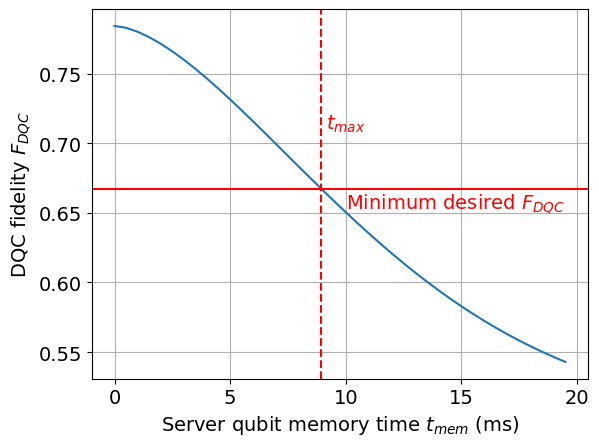
\includegraphics[width=0.48\linewidth]{figures/qnodeos/supplementary/plots/fidelity_vs_idle_time.png}}}%
    \hfill
    \subfloat[\centering \label{qnodeos:fig:delcomp-fidelity-alpha-colormap}]{{
        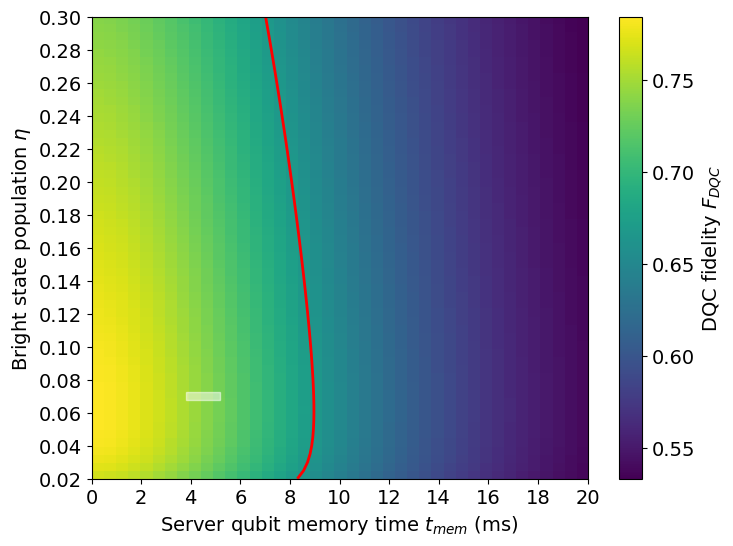
\includegraphics[width=0.48\linewidth]{figures/qnodeos/supplementary/plots/fidelity_eta_colormap.png}}}%
    \caption{
        (a) Expected values (based on simulation, \cref{qnodeos:sec:dqc-simulation}) of \ac{DQC} fidelity $F_{\text{DQC}}$ for different duration values that the server qubit must remain in memory ($t_{\text{mem}}$). The maximum allowed qubit memory time $t_{\max}$ is chosen such that application iterations that are expected to result in too low $F_{\text{DQC}}$ ($<0.667$) are filtered out.
        (b) Expected values (based on simulation) of \ac{DQC} fidelity $F_{\text{DQC}}$ for different values of the bright state population ($\eta$) in the single click protocol, and for different duration values that the server qubit must remain in memory ($t_{\text{mem}}$). The red line indicates the threshold of 0.667 for the target fidelity. The white box represents the experimentally obtained results (we fixed $\eta = 0.07$ and observed $t_{\text{mem}} ~4.8(8)$\,ms, see \cref{qnodeos:fig:fig3}d).
    }
    \label{qnodeos:fig:delcomp-simulation}
\end{figure*}

\subsection{Sweep of Qubit Memory Time and Bright State Population}

As explained in \cref{qnodeos:sec:NVentanglement}, entanglement is created using the single-photon protocol using bright state population parameter $\eta$.\footnote{In most literature, the variable $\alpha$ is used for this parameter; here we use $\eta$ to avoid confusion with the $\alpha$ parameter of the \ac{DQC} application.} Using the simulation, we can estimate how $F_{\text{DQC}}$ would change for different values of $\eta$ and $t_{\text{mem}}$. \cref{qnodeos:fig:delcomp-fidelity-alpha-colormap} shows the estimated $F_{\text{DQC}}$ for different values of $\eta$ and $t_{\text{mem}}$. It indicates that for the particular setup used, increasing $\eta$ has little effect, while reducing qubit memory time does. For the \ac{DQC} experiment $\eta = 0.07$ was used.

\subsection{Processing Time and Latencies}
\label{qnodeos:sec:processing_time_latencies}

Here we provide a detailed breakdown of the duration of execution phases of the \ac{DQC} application, in order to gain insights into the processing times and latencies of the system for the different components.

\subsubsection{Server qubit memory time}
\label{qnodeos:sec:server-qubit-memory-time}

\Cref{qnodeos:fig:fig3}c shows the duration that the server qubit must remain in memory $t_{\text{mem}}$ while waiting, averaged over all \ac{DQC} circuit iterations that passed the latency filter. \Cref{qnodeos:fig:fig3}d shows the breakdown of $t_{\text{mem}}$ into individual segments of processing on both client and server. In \cref{qnodeos:fig:delcomp-latencies-variance} we show the average duration and the variance of each of these segments. The largest time is spent on preparing S2, which involves running Python code on the \ac{CNPU} and converting this (using Python) into a \ac{NetQASM} subroutine. Caching of the preparation of the \ac{NetQASM} subroutine could significantly speed up this process. In the future, further improvements could include an optimized ahead-of-time compilation step. The large variance is due to the fact that on the \ac{CNPU}, other (background) processes run simultaneously with the \ac{DQC} application process, and there is no precise control over the scheduling of these processes.

\begin{figure*}[htbp]
\centering
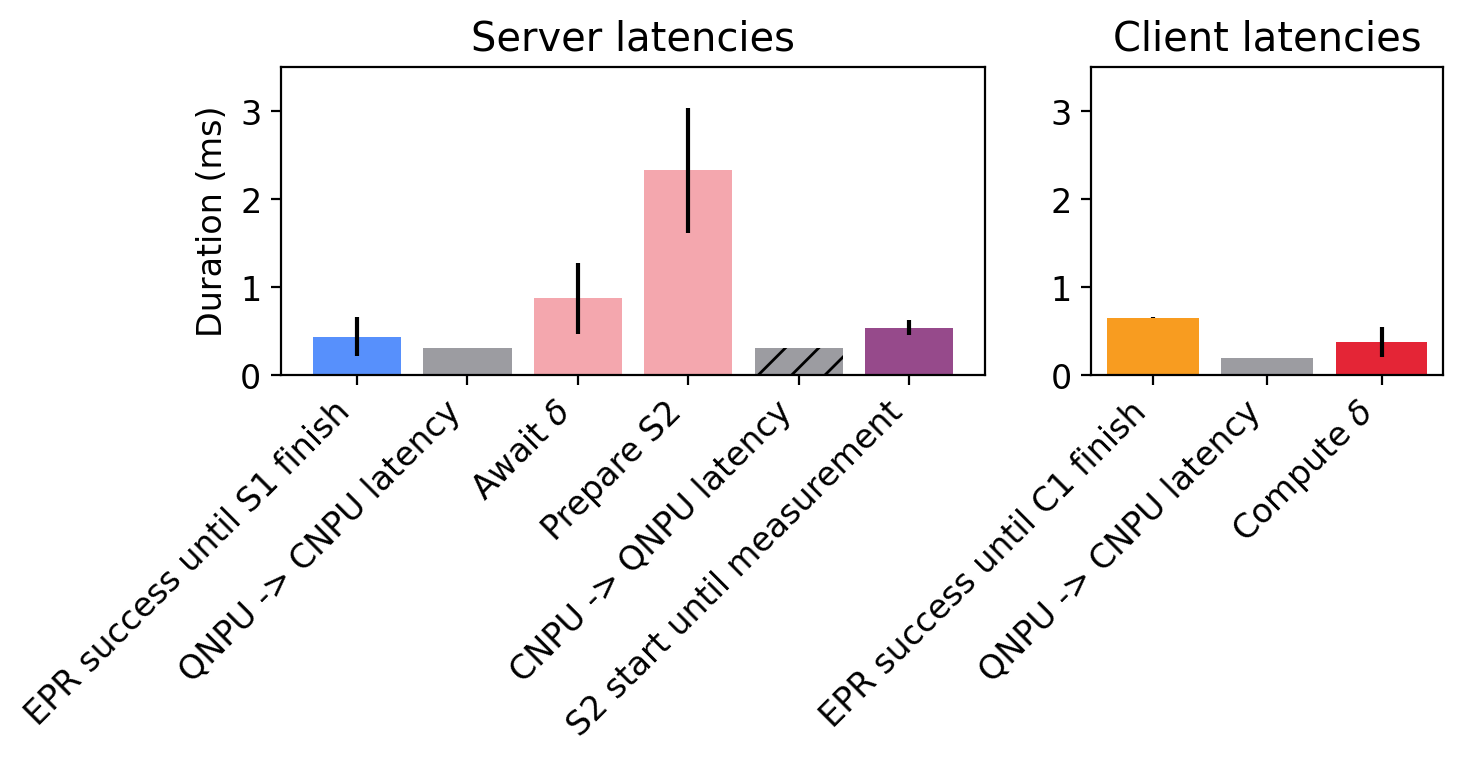
\includegraphics[width=0.8\linewidth]{figures/qnodeos/supplementary/plots/latencies_variance.png}
\caption{Average latency (duration) of each of the processes happening while the server qubit remains in memory in the \ac{DQC} application. The \ac{QNPU} to \ac{CNPU} latency and \ac{CNPU} to \ac{QNPU} latency are estimated as explained in \cref{qnodeos:sec:cnpu-qnpu-latency-estimation}, and fixed to 0.305\,ms (server) and 0.197\,ms (client). The other latencies are the mean and variance of the corresponding processes averaged over all \ac{DQC} circuit iterations that passed the latency filter.}
\label{qnodeos:fig:delcomp-latencies-variance}
\end{figure*}

\subsubsection{Tracing}

The \ac{CNPU}, \ac{QNPU}, and \ac{QDevice} all keep track of events happening in their system, by storing a tuple $(t, e)$ where $t$ is a timestamp and $e$ the name of the event. The events that are traced on the \ac{CNPU} and \ac{QNPU} are listed in \cref{qnodeos:sec:traces}. A trace plot showing events in \ac{CNPU}, \ac{QNPU}, and \ac{QDevice} during a single execution of the \ac{DQC} circuit is also shown in \cref{qnodeos:sec:traces}.

The \ac{QNPU} timestamp granularity is 10\,$\mu$s, since that is the duration of a single \ac{QNPU} clock cycle. This clock cycle is synchronized with the clock of the \ac{QDevice}, which in turn is synchronized with the \ac{QDevice} of the other node (see \cref{qnodeos:sec:methods} and all paragraphs therein related to \ac{NV} implementation). This results in the two \acp{QNPU} (of the two nodes in the experiment) having synchronized clocks with 10\,$\mu$s precision. This means that the event indicating to the \acp{QNPU} that \ac{EPR} generation has succeeded happens at the same clock cycle on both \acp{QNPU}.

The \ac{CNPU} is not a real-time system (instead, it runs on a general purpose Linux \ac{OS}) and records timestamps by consulting the system clock at $\mu$s precision. These timestamps are not synchronized to the \ac{QNPU} timestamps. Furthermore, the \ac{CNPU} timestamps obtained in this way are not as consistent as the real-time clock ticks on the \ac{QNPU}. Therefore, the relative \ac{CNPU} time compared to the \ac{QNPU} time (on the same node) may fluctuate.

% This involves two parts: (1) estimating the global timing offset $G$ between CNPU timestamps and QNPU timestamps, and (2) estimating the latency $L$ between the CNPU and QNPU. The following steps are done:

% \begin{itemize}
%     \item Comparing the difference between the first CNPU \texttt{subroutine sent" event and the first QNPU "subroutine added" event (which should $L + G$)
%     \item Comparing the difference between the first CNPU "result received" event and the first QNPU "subroutine done" event (which should also be $L + G$).
% \end{itemize}

% The average CNPU<->QNPU latency $L$ is then calculated as the average of
% \begin{itemize}
%     \item the global time difference found for the "subroutine send/added" events
%     \item the global time difference found for the "subroutine done/result received" events
% \end{itemize}

\subsubsection{CNPU-QNPU communication latency}
\label{qnodeos:sec:cnpu-qnpu-latency-estimation}

The latency of communication between the \ac{CNPU} and \ac{QNPU} can be calculated by looking at the time between \ac{CNPU} events and \ac{QNPU} events. However, since the \ac{CNPU} timestamps are fluctuating compared to the \ac{QNPU} timestamps, we cannot use a direct comparison between \ac{CNPU} and QNPU timestamps. Instead, we look at time differences on the \ac{CNPU} and compare them to time differences on the QNPU, given that we know the order in which events occur during the DQC application execution. \cref{qnodeos:fig:cnpu_qnpu_latencies} shows a schematic overview of events happening on the \ac{CNPU} and the \ac{QNPU} during a single execution of the \ac{DQC} circuit. By comparing, e.g., (1) the time difference on the \ac{CNPU} between sending subroutine S1 and receiving its result with (2) the time difference on the \ac{QNPU} between receiving subroutine S1 and finishing it, we can estimate the total latency of sending S1 from \ac{CNPU} to \ac{QNPU} and receiving its result. Using this technique, we can estimate the latencies for each communication between \ac{CNPU} and \ac{QNPU}, as listed in \cref{tab:delta_diffs}. Again, since the \ac{CNPU} timestamps fluctuate compared to the \ac{QNPU} timestamps, the derived latencies fluctuate and can even be negative. However, for all derived latencies, we found that a constant function best fit the data. This verifies that the actual latency is constant as expected, and that the variance is due to the inaccuracy of \ac{CNPU} timestamps.

\begin{table*}
    \centering
    \begin{tabular}{|c|c|c|}
    \hline
    \textbf{Derived latency (fit)} & \textbf{Description} & \textbf{Value (ms)} \\ 
    \hline
    $\Delta_{cS1} - \Delta_{qS1}$   & Send S1 + receive S1 result  & $0.384$ \\
    $\Delta_{qS12} - \Delta_{cS12}$ & Receive S1 result + Send S2  & $0.609$ \\
    $\Delta_{cS2} - \Delta_{qS2}$   & Send S2 + receive S2 result  & $0.467$ \\
    $\Delta_{cC1} - \Delta_{qC1}$   & Send C1 + receive C1 result  & $0.394$ \\
    \hline
    \end{tabular}
    \caption{Derived values for \ac{CNPU}-\ac{QNPU} communication latencies. The $\Delta$ variables are observed timestamp differences on the \ac{CNPU} or \ac{QNPU}, per execution of the \ac{DQC} circuit, as shown in \cref{qnodeos:fig:cnpu_qnpu_latencies}. Subtracting pairs of variables from each other produces sums of two \ac{CNPU}-\ac{QNPU} communication latencies. These sums of latencies highly fluctuate per execution of the \ac{DQC} circuit, due to the inaccuracy of the \ac{CNPU} timestamps. However, the data fits a constant value, which is shown in the table and used in further analysis.}
    \label{tab:delta_diffs}
\end{table*}

Using the result from \cref{tab:delta_diffs}, we can compute bounds on the four individual latency variables of the server (we have a system of three linear equations, and we know that all latencies must be strictly non-negative):
%
\begin{itemize}
    \item Sending S1 from \ac{CNPU} to \ac{QNPU}: $<$ 0.242\,ms.
    \item Receiving S1 result on \ac{CNPU} from \ac{QNPU}: between 0.142 and 0.384\,ms.
    \item Sending S2 from \ac{CNPU} to \ac{QNPU}: between 0.225 and 0.467\,ms.
    \item Receiving S2 result on \ac{CNPU} from QNPU: $<$ 0.242\,ms.
\end{itemize}

In the latency breakdown of the server qubit memory time (see \cref{qnodeos:sec:server-qubit-memory-time}) we are only interested in the latencies that happen during the time that the server qubit is in memory. For the server these are the latencies for receiving the S1 result and sending S2. The sum of these two latencies is $\Delta_{qS12} - \Delta_{cS12} = 0.609$\,ms (see \cref{tab:delta_diffs}). For simplicity, we say that both latencies constitute half of this time, as mentioned in the caption of \cref{qnodeos:fig:delcomp-latencies-variance}. Similarly, for the client we are only interested in the latency of receiving the C1 result. For simplicity we take this latency to be the same as that of sending C1, i.e. we use half of $\Delta_{cC1} - \Delta_{qC1}$.

\begin{figure*}[htbp]
    \centering
    \subfloat[\centering \label{qnodeos:fig:subfig3}]{{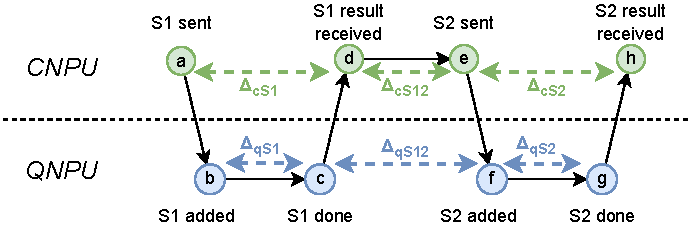
\includegraphics[width=0.61\linewidth]{figures/qnodeos/supplementary/host_qnpu_latency_server.pdf}}}%
    \hfill
    \subfloat[\centering \label{qnodeos:fig:subfig4}]{{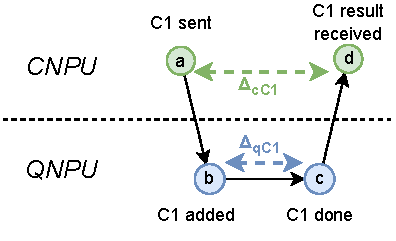
\includegraphics[width=0.35\linewidth]{figures/qnodeos/supplementary/host_qnpu_latency_client.pdf}}}%
    \caption{Schematic of events happening on the \ac{CNPU} and \ac{QNPU} during a single execution of \ac{DQC} on the server (a) and the client (b). Time flows to the right. The $\Delta$ variables are the time differences between events, and are used to estimate \ac{CNPU}-\ac{QNPU} communication latencies ($a\rightarrow b$, $c\rightarrow d$, $e\rightarrow f$, $g\rightarrow h$ on the server and $a\rightarrow b$, $c\rightarrow d$ on the client).}
    \label{qnodeos:fig:cnpu_qnpu_latencies}%
\end{figure*}

\subsubsection{Entanglement generation}

An overview of all values discussed in this section is given in \cref{tab:entanglement_stats}.

\ac{EPR} generation happens by attempting entanglement repeatedly until success. The \ac{QNPU} sends an \texttt{ENT} physical instruction (\cref{tab:qdevice-instructions}) to the \ac{QDevice}, which starts a batch of physical attempts. Each attempt takes 3.95\,$\mu$s and a batch contains 500 attempts. If a batch fails (no success after 500 attempts), the \ac{QNPU} sends another \texttt{ENT} instruction. \cref{tab:entanglement_stats} lists the average success probability per attempt and per batch that we found in the \ac{DQC} experiments. As explained in \cref{qnodeos:sec:NVentanglement}, the \ac{NV} \ac{QDevice} creates either a $\Psi^+$ or a $\Psi^-$ state. \Cref{tab:entanglement_stats} shows statistics on how often each of these states was created during our experiments.

\cref{qnodeos:fig:delcomp-epr-rate} shows the distribution of time it takes to generate an \ac{EPR} pair in the \ac{DQC} experiment, where the average duration of such is 439\,ms. This is the duration between starting the network process and finishing it, which includes entanglement attempts until success on the \ac{QDevice} and subsequent Bell state corrections to $\Phi^+$ (see \cref{qnodeos:sec:qdevice-nv}). This duration corresponds to a fitted rate of 2.28(3) created \ac{EPR} pairs per second. If only the \ac{QDevice} entanglement generation is considered (i.e. without Bell state corrections and without \ac{QNPU} processing overhead), this rate is 2.37(2) \ac{EPR} pairs per second.

\begin{figure}
\centering
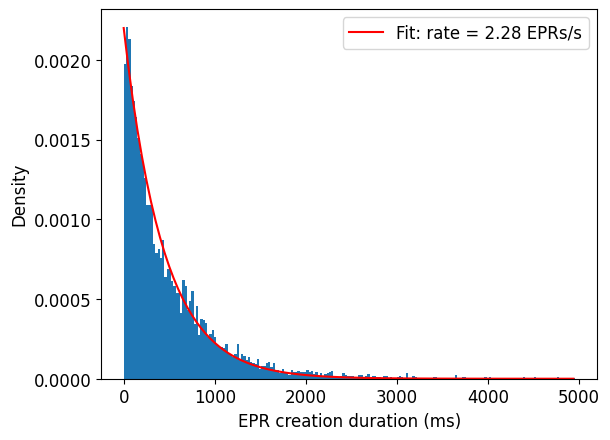
\includegraphics[width=\linewidth]{figures/qnodeos/supplementary/plots/EPR_rate.png}
\caption{Histogram of \ac{EPR} generation durations (time from first attempt until success) based on all \ac{EPR} generations in the \ac{DQC} experiment (using only latency-filtered data points, see \cref{qnodeos:sec:post-selection-latency}). The histogram shows which fraction of all durations were in a particular duration window (window width: 25\,ms). Expected \ac{EPR} generation duration follows an exponential decay, with a rate parameter of 2.28(3) successes (\ac{EPR} pairs) per second.}
\label{qnodeos:fig:delcomp-epr-rate}
\end{figure}

\begin{table*}[htpb]
    \centering
    \begin{tabular}{|r|l|}
    \hline
    \textbf{Parameter} & \textbf{Value} \\ 
    \hline
    Duration of a single entanglement attempt* & 3.95\,$\mu$s \\
    Number of attempts per batch* & 500 \\
    Average number of failed batches until success & 144 \\
    Average success probability per batch & $6.95 \times 10^{-3}$ \\
    Average success probability per attempt & $1.39 \times 10^{-5}$ \\
    Number of Psi+ states generation & 3187 (44.3\%) \\
    Number of Psi- states generation & 4013 (55.7\%) \\
    EPR generation rate (fit) (QDevice) & 2.37(2) EPRs/s \\
    EPR generation rate (fit) (QNodeOS) & 2.28(3) EPRs/s \\
    Average fraction of EPR generation time spent on sync failure & 0.18 \\
    % ...of which client fraction & 0.54 \\
    % ...of which server fraction & 0.46 \\
    
    \hline
    \end{tabular}
    \caption{Overview of values derived from the \ac{DQC} experiment analysis, based on all 7200 \ac{DQC} circuit executions. Entries with an asterisk (*) are values that we fixed in our experiments. The other values are observed experimental results. Average success probabilities are derived from the number of failed batches until success.
    \ac{EPR} generation rate is distinguished between \ac{QDevice} and \ac{QNodeOS}. For the \ac{QDevice}, it indicates the fitted (to an exponential decay function) time between the first \texttt{ENT} physical instruction and the first entanglement success (see \cref{qnodeos:sec:appendix-qdevice}). For \ac{QNodeOS}, it indicates the fitted time between the start of the network process and the end of the network process (i.e. when entanglement has been created and Bell state corrections have been applied, see \cref{qnodeos:sec:qdevice-nv}). Entanglement sync failures happen when one \ac{QDevice} (server or client) wants to attempt entanglement but the other \ac{QDevice} is not ready (\cref{qnodeos:sec:qdevice-sync}). Such sync failures were observed intermittently during a batch of entanglement attempts.}
    \label{tab:entanglement_stats}
\end{table*}

\subsubsection{Local gate durations}

As part of the \ac{DQC} execution, the \ac{QNPU} sends physical instructions to the \ac{NV} \ac{QDevice} for executing local quantum gates. In \cref{tab:gate_durations} we report on the observed durations of these gates from the perspective of the \ac{QNPU}: these durations are from the time the physical instruction is sent to the \ac{QDevice} until the corresponding result is received from the \ac{QDevice}. We note that these durations are longer than these gates would take if they were executed directly on the \ac{QDevice} (without \ac{QNodeOS}, see \cref{tab:mw_pulse}) because of two reasons: (1) the limited granularity with which the \ac{QNPU} and \ac{QDevice} communicate (rounds of 10\,$\mu$s) and (2) the fact the \ac{QDevice} interleaves \ac{DD} sequences in between sequences for the physical instruction itself, as explained in \cref{qnodeos:sec:methods}.

\begin{table*}
    \centering
    \begin{tabular}{|c|c|c|}
    \hline
    \textbf{Physical instruction} & \textbf{Duration (client)} & \textbf{Duration (server)} \\ 
    \hline
    Measure & 130--160\,$\mu$s & 80 - 100\,$\mu$s \\
    X90 & 80--100\,$\mu$s & 50 - 130\,$\mu$s \\
    X180 & 80--100\,$\mu$s & 10 - 130\,$\mu$s \\
    -X90 & --- & 50 - 130\,$\mu$s \\
    Y90 & 70--200\,$\mu$s & 50 - 130\,$\mu$s \\
    Y90 & --- & 50 - 130\,$\mu$s \\
    \hline
    \end{tabular}
    \caption{Duration of executing local quantum gates on the \ac{NV} \ac{QDevice} in the \ac{DQC} experiment. Durations are from sending the physical instruction from \ac{QNPU} to \ac{QDevice} until receiving the \ac{QDevice} response. The -X90 and Y90 gates were never executed in the client \ac{DQC} program.}
    \label{tab:gate_durations}
\end{table*}

\subsubsection{General experiment statistics}

\cref{tab:exp_durations} lists statistics about the overall \ac{DQC} experiment (all 7200 \ac{DQC} circuit executions combined). We confirm our hypothesis that the overwhelming fraction of time is spent on the network process, namely generating \ac{EPR} pairs. We also see that as expected, the server spends more time on user processes than the client does, since it does more local gates than the client (namely, the gates in subroutine S2).

\begin{table*}[htpb]
    \centering
    \begin{tabular}{|r|c|c|}
    \hline
    \textbf{Value} & \textbf{Client} & \textbf{Server} \\ 
    \hline
    Total experiment duration & 4243\,s & 4065\,s \\
    Time spent executing network process & 3840\,s & 3825\,s \\
    Time spent executing user processes & 5.041\,s & 7.618\,s \\
    \hline
    \end{tabular}
    \caption{Overall durations of the \ac{DQC} experiment.}
    \label{tab:exp_durations}
\end{table*}

\subsection{QNPU Network process analysis}

In this section we focus on the execution of the network process in the \ac{QNPU} as observed in the execution of \ac{DQC}. The \ac{ER} sockets (\cref{qnodeos:sec:design_er_socket}) are designed to facilitate the generation of entanglement belonging to a pair of user processes between two different \acp{QNPU}. In particular, the \ac{ER} socket allows the \ac{QNPU} to proceed with entanglement generation, while only one node may not have issued a request for entanglement yet. 

During execution of the \ac{DQC} application, the client \ac{QNPU} has a single user process $P_c$ for its \ac{DQC} program and the server \ac{QNPU} has a single user process $P_s$ for its \ac{DQC} program. Both user processes realize the repeated execution of subroutines that jointly realize the \ac{DQC} circuit (\cref{qnodeos:fig:fig3}a).

In each single repetition of the \ac{DQC} circuit, $P_s$ executes first S1 and then S2, and $P_c$ executes C1. $P_s$ (in S1) and $P_c$ (in C1) execute a \ac{NetQASM} instruction for creating an entangled pair, which results in an entanglement request that is submitted to the network stack. Then, $P_c$ and $P_s$ go into the waiting state (see \cref{qnodeos:sec:design:processes}) until the entangled pair is delivered by the network process.

$P_c$ executes a \texttt{create\_epr} instruction and $P_s$ executes a \texttt{recv\_epr} instruction (determined by program source code, see \cref{qnodeos:sec:app_source}. Therefore, the client is seen as the \emph{initiator} (see \cref{qnodeos:sec:design_er_socket}). $P_s$ and $P_c$ open a pair of \ac{ER} sockets with each other when they start and keep it open for the whole experiment. $P_c$ and $P_s$, being on different nodes, operate independently, and may hit their entanglement request instruction at different times. Since the client is the initiator and the server the receiver, the server is always willing to handle an entanglement request with the client. So, the network stack on both client and server will handle a request for entanglement as soon as the client submitted it to its network stack, regardless of whether the server already executed the corresponding \texttt{recv\_epr} in S1.

We observe that in 3245 out of all 7200 \ac{DQC} circuit executions, the client submitted the corresponding entanglement request to its network stack (in C1) \textit{before} the server submitted its entanglement request to its own network stack (in S1), but where the server still complied by starting the network process and handling the request.

\subsubsection{Client waits for server}

From our architecture, we expect that it can happen that the client must wait for the server. This can be the case in the following scenario: The client executes C1 for \ac{DQC} circuit iteration $i$ and submits the entanglement request. Then, the next network time bin starts and the client \ac{QNPU} starts the network process. However, the server is at this time (the beginning of the time bin) still busy with executing S2 for iteration $i-1$ (in user process $P_s$). Therefore the server \ac{QNPU} cannot yet activate its own network process. Since the \ac{ER} socket with the server is open and the client is the `initiator', the client will send entanglement physical instructions to the \ac{QDevice} anyway, but the \ac{QDevice} will not be able to do actual attempts because the server \ac{QDevice} is not ready (\cref{qnodeos:sec:qdevice-sync}). Only when the server \ac{QNPU} completes S2, it can activate the network process, which then sends entanglement physical instructions to the \ac{QDevice}. Only at this point the \acp{QDevice} can start actual entanglement generation. We observe that it did indeed happen that the client had to wait for the server, although we observed this behavior in only in 60 out of 7200 \ac{DQC} circuit executions.

\subsubsection{Server waits for client}

We expect that it can also happen that the server must wait for the client. This can be the case in the following scenario: The server executes S1 for \ac{DQC} circuit iteration $i$ and submits the entanglement request. Then, the next network time bin starts. However, the client did not yet hit the entanglement request in C1 for \ac{DQC} iteration $i$, so there is nothing to do for the server network process. The server hence needs to wait for the next time-bin, and check again if by now the client has submitted its entanglement request. We observe that in 1323 out of 7200 \ac{DQC} circuit executions, the server had to wait for the client.

\subsubsection{Start of network process}

We examine the start of the network process in relation to the start of a time bin. In particular, the start of the network process may be delayed if there is still a user process running. 

The network process is only activated at the beginning of a time bin. In our experiment, a time bin starts every 10\,ms and lasts 10\,ms. In most cases when the network process is activated, this activation happens very quickly after the time bin start (within 100\,$\mu$s, as some \ac{QNPU} software processing is needed). For the client \ac{QNPU}, the network process never starts more than 100\,$\mu$s after a time bin start. For the server, in 13 out of 7200 \ac{DQC} circuit executions, the network process starts more than 100\,$\mu$s after a time bin starts, since in these cases there was still a user process running. In \cref{tab:network_process_stats}, an overview of all network process statistics is given.

\begin{table*}
    \centering
    \begin{tabular}{|l|l|}
    \hline
    \textbf{Parameter} & \textbf{Value} \\ 
    \hline
    Number of times server puts \ac{EPR} request to network stack before client & 1774/7200 \\
    Number of times server starts entanglement before putting in \ac{EPR} request & 3245/7200 \\
    Number of times submitted \ac{EPR} request is handled in immediate next time bin & 5523/7200 \\
    Average number of bins that pass before request is handled & 2.33 \\
    Number of times server needs to wait for client & 1323/7200 \\
    Number of times client needs to wait for server & 60/7200 \\
    Number of times client network process starts > 100\,$\mu$s after time bin starts & 0 \\
    Number of times server network process starts > 100\,$\mu$s after time bin starts & 13 \\
    \hline
    \end{tabular}
    \caption{Statistics on the \ac{QNPU} network process behavior during the whole \ac{DQC} experiment, i.e. totalled over all 7200 \ac{DQC} circuit iterations.}
    \label{tab:network_process_stats}
\end{table*}